\documentclass[border=12pt]{standalone}
\usepackage{tikz}
\usetikzlibrary{shapes.geometric, arrows.meta, positioning, calc, fit, backgrounds}
\usepackage{fontspec}
\usepackage{amsmath}
\setmainfont{DejaVu Sans}

\begin{document}
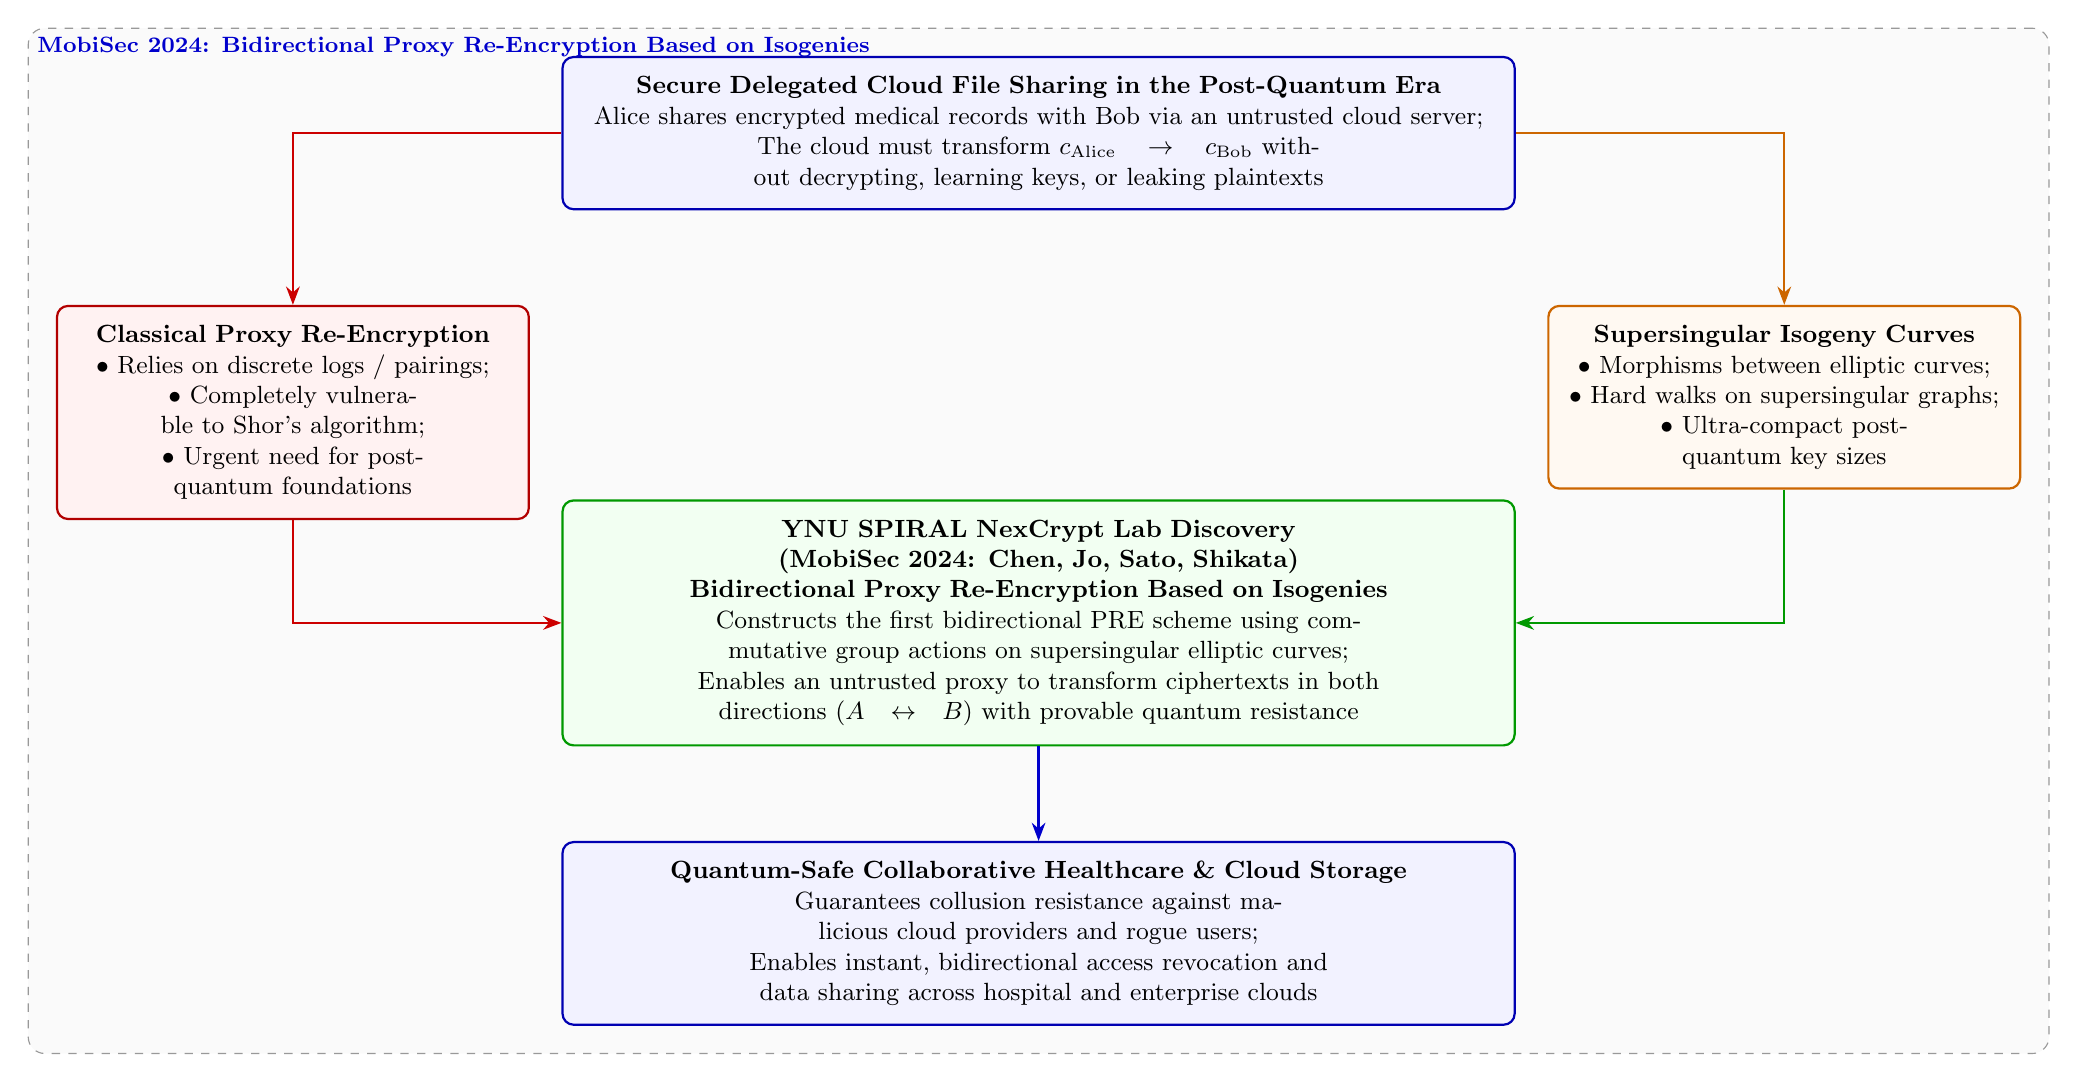
\begin{tikzpicture}[
    font=\small,
    >=Stealth,
    node distance=1.2cm,
    block/.style={rectangle, draw=blue!70!black, fill=blue!5, rounded corners=4pt, thick, align=center, inner sep=7pt},
    alertblock/.style={rectangle, draw=red!70!black, fill=red!5, rounded corners=4pt, thick, align=center, inner sep=7pt},
    greenblock/.style={rectangle, draw=green!60!black, fill=green!5, rounded corners=4pt, thick, align=center, inner sep=7pt},
    amberblock/.style={rectangle, draw=orange!80!black, fill=orange!5, rounded corners=4pt, thick, align=center, inner sep=7pt},
    groupbox/.style={draw=black!40, dashed, rounded corners=6pt, fill=black!2, inner sep=10pt}
]

    % Top: The Post-Quantum Cloud Data Sharing Challenge
    \node[block, text width=11.6cm] (cloud) {\textbf{Secure Delegated Cloud File Sharing in the Post-Quantum Era}\\Alice shares encrypted medical records with Bob via an untrusted cloud server;\\The cloud must transform $c_{\text{Alice}} \to c_{\text{Bob}}$ without decrypting, learning keys, or leaking plaintexts};

    % Left: Traditional Discrete-Log PRE Vulnerability
    \node[alertblock, below left=1.2cm and 0.4cm of cloud, text width=5.5cm] (vulnerable) {\textbf{Classical Proxy Re-Encryption}\\$\bullet$ Relies on discrete logs / pairings;\\$\bullet$ Completely vulnerable to Shor's algorithm;\\$\bullet$ Urgent need for post-quantum foundations};

    % Right: Isogeny Graph Geometry
    \node[amberblock, below right=1.2cm and 0.4cm of cloud, text width=5.5cm] (isogeny) {\textbf{Supersingular Isogeny Curves}\\$\bullet$ Morphisms between elliptic curves;\\$\bullet$ Hard walks on supersingular graphs;\\$\bullet$ Ultra-compact post-quantum key sizes};

    \draw[->, thick, red!80!black] (cloud) -| (vulnerable);
    \draw[->, thick, orange!80!black] (cloud) -| (isogeny);

    % Middle: YNU Discovery (MobiSec 2024: Chen, Jo, Sato, Shikata)
    \node[greenblock, below=1.2cm of $(vulnerable)!0.5!(isogeny)$, text width=11.6cm] (breakthrough) {\textbf{YNU SPIRAL NexCrypt Lab Discovery (MobiSec 2024: Chen, Jo, Sato, Shikata)}\\\textbf{Bidirectional Proxy Re-Encryption Based on Isogenies}\\Constructs the first bidirectional PRE scheme using commutative group actions on supersingular elliptic curves;\\Enables an untrusted proxy to transform ciphertexts in both directions ($A \leftrightarrow B$) with provable quantum resistance};

    \draw[->, thick, red!80!black] (vulnerable) |- (breakthrough);
    \draw[->, thick, green!60!black] (isogeny) |- (breakthrough);

    % Bottom: Impact
    \node[block, below=1.2cm of breakthrough, text width=11.6cm] (impact) {\textbf{Quantum-Safe Collaborative Healthcare \& Cloud Storage}\\Guarantees collusion resistance against malicious cloud providers and rogue users;\\Enables instant, bidirectional access revocation and data sharing across hospital and enterprise clouds};

    \draw[->, thick, blue!80!black] (breakthrough) -- (impact);

    \begin{scope}[on background layer]
        \node[groupbox, fit=(cloud) (vulnerable) (isogeny) (breakthrough) (impact), label={[anchor=north west, font=\footnotesize\bfseries, blue!80!black]north west:MobiSec 2024: Bidirectional Proxy Re-Encryption Based on Isogenies}] {};
    \end{scope}

\end{tikzpicture}
\end{document}
